\documentclass[10pt,a4paper]{article}
\usepackage[a4paper,margin=1.7cm]{geometry}
\usepackage{fontspec}
\usepackage{booktabs}
\usepackage{tabularx}
\usepackage{xcolor}
\usepackage{fancyhdr}
\usepackage{listings}
\usepackage{titlesec}
\usepackage{tikz}
\usepackage{hyperref}
% Shared TikZ styles for the Maestro design-document figures.
\usetikzlibrary{positioning,calc,fit,backgrounds,arrows.meta}

\tikzset{
  win/.style        = {draw=black!60, rounded corners=2pt, fill=white, line width=0.5pt},
  titlebar/.style   = {draw=black!60, fill=black!10, rounded corners=2pt, line width=0.5pt},
  strip/.style      = {draw=black!35, fill=black!4, line width=0.4pt},
  panel/.style      = {draw=black!40, fill=black!2, rounded corners=1.5pt, line width=0.4pt},
  panelhdr/.style   = {font=\scriptsize\bfseries, anchor=west, text=black!75},
  tab/.style        = {draw=black!40, fill=black!5, rounded corners=1.5pt, font=\scriptsize, inner sep=2pt, line width=0.4pt},
  tabsel/.style     = {draw=black!70, fill=black!20, rounded corners=1.5pt, font=\scriptsize\bfseries, inner sep=2pt, line width=0.6pt},
  btn/.style        = {draw=black!50, fill=black!8, rounded corners=1.5pt, font=\scriptsize, inner sep=2.5pt, line width=0.4pt},
  field/.style      = {draw=black!45, fill=white, rounded corners=1pt, font=\scriptsize\ttfamily, inner sep=2.5pt, line width=0.4pt},
  mono/.style       = {font=\scriptsize\ttfamily, anchor=west, inner sep=0pt},
  monos/.style      = {font=\tiny\ttfamily, anchor=west, inner sep=0pt},
  monob/.style      = {font=\scriptsize\ttfamily\bfseries, anchor=west, inner sep=0pt},
  lbl/.style        = {font=\scriptsize, anchor=west, inner sep=0pt},
  note/.style       = {font=\scriptsize\itshape, anchor=west, text=black!55, inner sep=0pt},
  callout/.style    = {font=\scriptsize\itshape, text=black!55, anchor=west},
  arrowto/.style    = {-{Latex[length=3pt]}, draw=black!45, line width=0.4pt},
  ok/.style         = {circle, fill=black!65, inner sep=1.1pt},
  warn/.style       = {draw=black!70, fill=black!25, rounded corners=1pt, font=\tiny\bfseries, inner sep=1.5pt},
}

% \gauge{x}{y}{width}{fraction}{label}
\newcommand{\gauge}[5]{%
  \draw[draw=black!45, fill=black!6, rounded corners=1pt] (#1,#2) rectangle ++(#3,0.22);
  \draw[draw=none, fill=black!55, rounded corners=1pt] (#1,#2) rectangle ++({#3*#4},0.22);
  \node[monos, anchor=west] at (#1+#3+0.1,#2+0.11) {#5};%
}

% \sparkline{x}{y}{unit width}{max height}{comma list of 0..1 values}
\newcommand{\sparkline}[5]{%
  \foreach \v [count=\i from 0] in {#5} {
    \draw[draw=none, fill=black!45] ({#1+\i*#3},#2) rectangle ++({#3*0.7},{#4*\v});
  }%
}

\hypersetup{colorlinks=true, linkcolor=black, urlcolor=blue!60!black}
\setmainfont{Georgia}
\setmonofont{Consolas}
% the document carries its own section numbers (1., 3.1, ...)
\setcounter{secnumdepth}{0}
\setcounter{tocdepth}{2}
% wireframes: never wrap, fixed columns, small enough to fit 100 cols
\lstset{
  basicstyle=\scriptsize\ttfamily,
  breaklines=false,
  columns=fixed,
  keepspaces=true,
  frame=single,
  framesep=3pt,
  xleftmargin=2pt,
  backgroundcolor=\color{gray!7},
  aboveskip=8pt, belowskip=8pt,
}
\titleformat{\section}{\large\bfseries}{}{0pt}{}
\titleformat{\subsection}{\normalsize\bfseries}{}{0pt}{}
\titleformat{\subsubsection}{\small\bfseries}{}{0pt}{}
\setlength{\parskip}{4pt}
\setlength{\parindent}{0pt}
\pagestyle{fancy}
\fancyhf{}
\fancyhead[L]{\small Maestro --- TUI Design}
\fancyhead[R]{\small\thepage}
\renewcommand{\headrulewidth}{0.4pt}
\title{\textbf{Maestro --- TUI Design}\\[2pt]
\large Wireframes, interaction flows and settings inventory}
\author{}
\date{}
\begin{document}
\maketitle
\thispagestyle{empty}
{\small\tableofcontents}
\clearpage
Companion to the design decisions (FR-10). All wireframes are schematic mock-ups of AppCUI windows/controls (rendered as vector figures in the PDF build). AppCUI model: a \textbf{desktop} hosts multiple \textbf{windows}; a bottom/top \textbf{app bar} shows global status; every action is reachable by keyboard, menu and mouse.

\section{1. Design Principles}
\begin{itemize}
  \item \textbf{One Mission Control, many satellites.} The main window (tabs) is for global state;
every \emph{project} and every \emph{session} can open as its own satellite window so parallel work is visible side by side on the desktop.

  \item \textbf{Live by default.} Every list/gauge subscribes to the event bus; no refresh buttons.
  \item \textbf{Nothing hidden.} Pending questions, write-queue depth and quota alarms are always
one glance away (app bar + dashboard ticker).

  \item \textbf{Keyboard-first.} Global hotkeys work from any window; every form is tab-navigable.
  \item \textbf{Same core for TUI and CLI} — the TUI is a view; \texttt{maestro-cli} can do everything.
\end{itemize}
\section{2. Global Chrome}
\begin{center}
% Global chrome: menu bar, desktop, app bar (TUI-DESIGN 2)
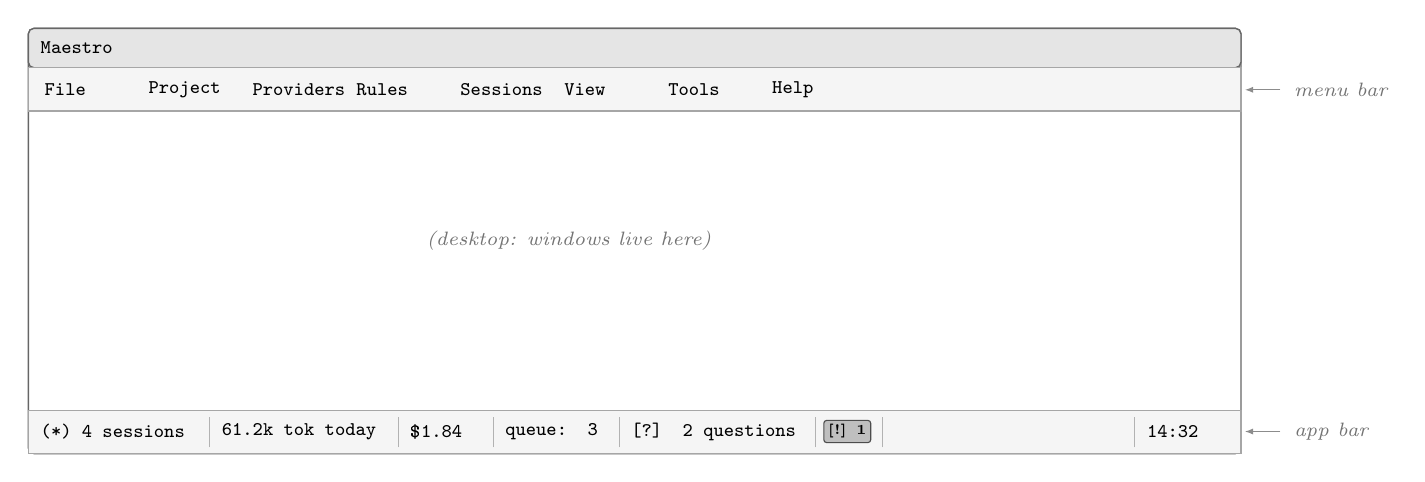
\begin{tikzpicture}[x=1cm,y=1cm]
  % window
  \draw[win] (0,0) rectangle (15.4,5.4);
  \draw[titlebar] (0,4.9) rectangle (15.4,5.4);
  \node[monob] at (0.15,5.15) {Maestro};

  % menu bar
  \draw[strip] (0,4.35) rectangle (15.4,4.9);
  \foreach \m [count=\i from 0] in {File,Project,Providers,Rules,Sessions,View,Tools,Help} {
    \node[mono] at ({0.2+\i*1.32},4.62) {\m};
  }

  % desktop
  \node[note] at (5.05,2.7) {(desktop: windows live here)};

  % app bar
  \draw[strip] (0,0) rectangle (15.4,0.55);
  \node[mono] at (0.15,0.28) {(*) 4 sessions};
  \node[mono] at (2.45,0.28) {61.2k tok today};
  \node[mono] at (4.85,0.28) {\$1.84};
  \node[mono] at (6.05,0.28) {queue: 3};
  \node[mono] at (7.65,0.28) {[?] 2 questions};
  \node[warn] at (10.4,0.28) {[!] 1};
  \node[mono] at (14.2,0.28) {14:32};
  \foreach \x in {2.3,4.7,5.9,7.5,10.0,10.85,14.05} {
    \draw[black!30, line width=0.3pt] (\x,0.08) -- (\x,0.47);
  }

  % callouts
  \draw[arrowto] (15.9,4.62) -- (15.45,4.62);
  \node[callout] at (15.95,4.62) {menu bar};
  \draw[arrowto] (15.9,0.28) -- (15.45,0.28);
  \node[callout] at (15.95,0.28) {app bar};
\end{tikzpicture}

\end{center}

\begin{itemize}
  \item \textbf{App bar segments} (left->right): active sessions • tokens today • cost today •
write-queue depth • pending clarifications (click -> Interrogation Center) • active alerts (click -> alerts log) • clock. Segments are clickable buttons.

  \item \textbf{Menu map}:
  \begin{itemize}
    \item \emph{File}: New Project, Open Workspace, Import/Export Config, Quit
    \item \emph{Project}: Run/Pause/Resume, New Task, Interview, Regenerate AGENTS.md, Skills…
    \item \emph{Providers}: Add Provider, Detect CLIs, Health Check All, Quota Report
    \item \emph{Rules}: New Rule, Dry-Run, Import YAML
    \item \emph{Sessions}: Quick Chat, New Task Session, Pause All, Transcripts…
    \item \emph{View}: Mission Control, Tile Windows, Theme, Focus Mode
    \item \emph{Tools}: Settings, Config Doctor, Logs, Sandbox Allow-Lists
    \item \emph{Help}: Shortcuts, About
  \end{itemize}
\end{itemize}
\section{3. Mission Control (main window, opens maximized)}
Tab control with 6 fixed tabs: \textbf{Dashboard · Projects · Providers · Rules · Questions · Activity}.

\subsection{3.1 Dashboard tab}
\begin{center}
% Mission Control - Dashboard tab (TUI-DESIGN 3.1)
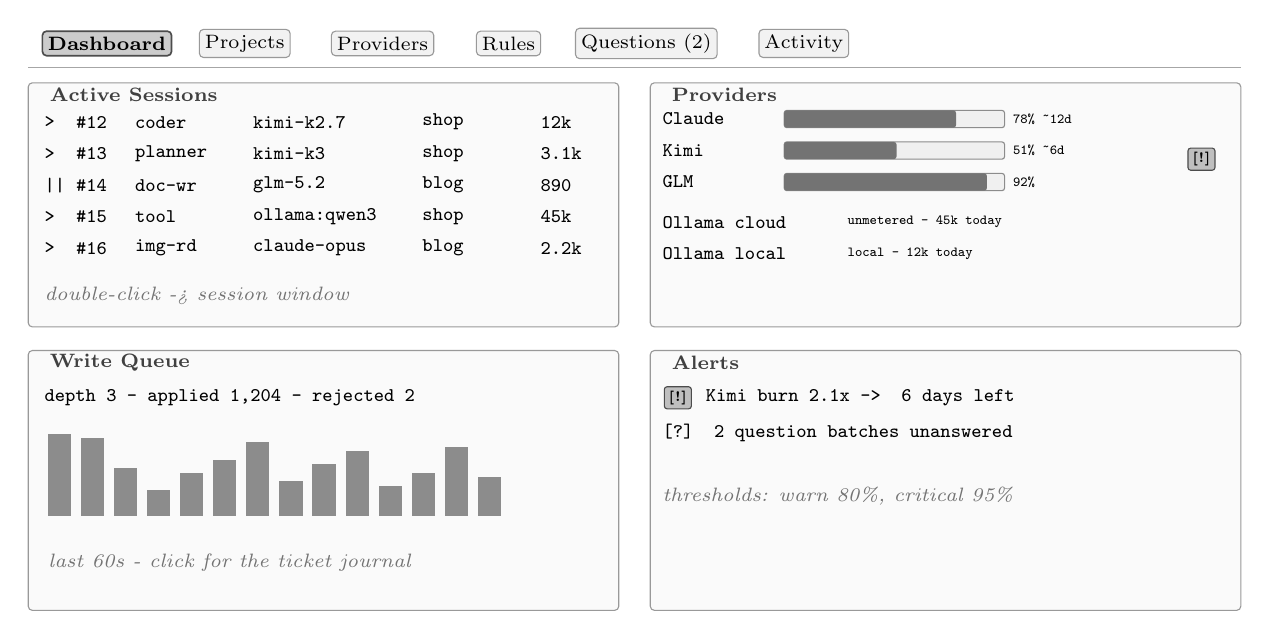
\begin{tikzpicture}[x=1cm,y=1cm]
  % tab strip
  \node[tabsel] at (1.0,7.35) {Dashboard};
  \foreach \t/\x in {Projects/2.75, Providers/4.5, Rules/6.1, {Questions (2)}/7.85, Activity/9.85} {
    \node[tab] at (\x,7.35) {\t};
  }
  \draw[black!35, line width=0.4pt] (0,7.05) -- (15.4,7.05);

  % ---------- Active sessions ----------
  \draw[panel] (0,3.75) rectangle (7.5,6.85);
  \node[panelhdr] at (0.15,6.7) {Active Sessions};
  \foreach \g/\id/\role/\model/\proj/\tok/\y in {%
    >/\#12/coder/kimi-k2.7/shop/12k/6.35,
    >/\#13/planner/kimi-k3/shop/3.1k/5.95,
    ||/\#14/doc-wr/glm-5.2/blog/890/5.55,
    >/\#15/tool/ollama:qwen3/shop/45k/5.15,
    >/\#16/img-rd/claude-opus/blog/2.2k/4.75}
  {
    \node[mono] at (0.2,\y) {\g};
    \node[mono] at (0.6,\y) {\id};
    \node[mono] at (1.35,\y) {\role};
    \node[mono] at (2.85,\y) {\model};
    \node[mono] at (5.0,\y) {\proj};
    \node[mono] at (6.5,\y) {\tok};
  }
  \node[note] at (0.2,4.15) {double-click -> session window};

  % ---------- Providers with quota gauges ----------
  \draw[panel] (7.9,3.75) rectangle (15.4,6.85);
  \node[panelhdr] at (8.05,6.7) {Providers};
  \foreach \n/\f/\l/\y in {%
    Claude/0.78/{78\% \textasciitilde 12d}/6.28,
    Kimi/0.51/{51\% \textasciitilde 6d}/5.88,
    GLM/0.92/{92\%}/5.48}
  {
    \node[mono] at (8.05,\y+0.11) {\n};
    \gauge{9.6}{\y}{2.8}{\f}{\l}
  }
  \node[mono] at (8.05,5.08) {Ollama cloud};
  \node[monos] at (10.4,5.08) {unmetered - 45k today};
  \node[mono] at (8.05,4.68) {Ollama local};
  \node[monos] at (10.4,4.68) {local - 12k today};
  \node[warn] at (14.9,5.88) {[!]};

  % ---------- Write queue ----------
  \draw[panel] (0,0.15) rectangle (7.5,3.45);
  \node[panelhdr] at (0.15,3.3) {Write Queue};
  \node[mono] at (0.2,2.85) {depth 3 - applied 1,204 - rejected 2};
  \sparkline{0.25}{1.35}{0.42}{1.1}{0.95,0.9,0.55,0.3,0.5,0.65,0.85,0.4,0.6,0.75,0.35,0.5,0.8,0.45}
  \node[note] at (0.25,0.75) {last 60s - click for the ticket journal};

  % ---------- Alerts ----------
  \draw[panel] (7.9,0.15) rectangle (15.4,3.45);
  \node[panelhdr] at (8.05,3.3) {Alerts};
  \node[warn] at (8.25,2.85) {[!]};
  \node[mono] at (8.6,2.85) {Kimi burn 2.1x -> ~6 days left};
  \node[mono] at (8.05,2.4) {[?] 2 question batches unanswered};
  \node[note] at (8.05,1.6) {thresholds: warn 80\%, critical 95\%};
\end{tikzpicture}

\end{center}

\begin{itemize}
  \item Sessions listview: double-click -> session window; right-click -> pause/steer/kill/migrate.
  \item Provider gauges: progress bars + projected-exhaustion estimate; click -> provider window.
  \item Write queue: depth + applied/rejected counters + sparkline (GraphView); click -> ticket log.
\end{itemize}
\subsection{3.2 Projects tab}
\begin{center}
% Mission Control - Projects tab (TUI-DESIGN 3.2)
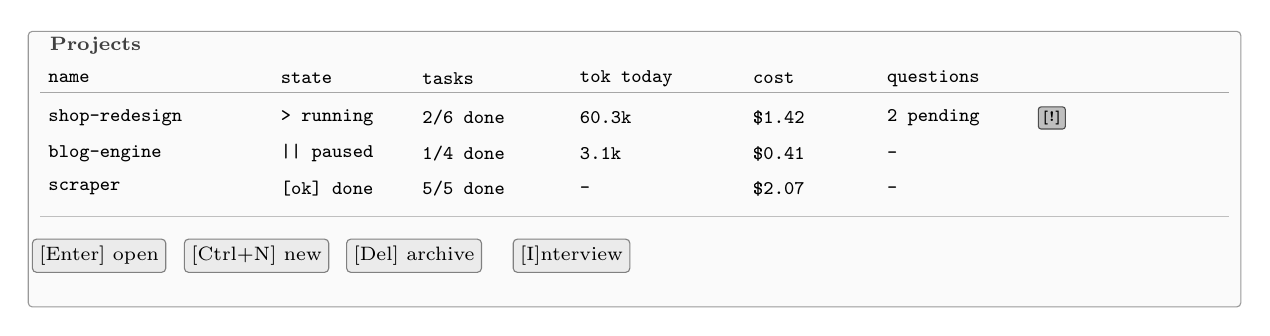
\begin{tikzpicture}[x=1cm,y=1cm]
  \draw[panel] (0,0) rectangle (15.4,3.5);
  \node[panelhdr] at (0.15,3.32) {Projects};

  % header row
  \foreach \h/\x in {name/0.25, state/3.2, tasks/5.0, {tok today}/7.0, cost/9.2, questions/10.9} {
    \node[monob] at (\x,2.9) {\h};
  }
  \draw[black!35, line width=0.4pt] (0.15,2.72) -- (15.25,2.72);

  \foreach \n/\s/\t/\k/\c/\q/\y in {%
    shop-redesign/{> running}/{2/6 done}/60.3k/{\$1.42}/{2 pending}/2.4,
    blog-engine/{|| paused}/{1/4 done}/3.1k/{\$0.41}/{-}/1.95,
    scraper/{[ok] done}/{5/5 done}/-/{\$2.07}/{-}/1.5}
  {
    \node[mono] at (0.25,\y) {\n};
    \node[mono] at (3.2,\y) {\s};
    \node[mono] at (5.0,\y) {\t};
    \node[mono] at (7.0,\y) {\k};
    \node[mono] at (9.2,\y) {\c};
    \node[mono] at (10.9,\y) {\q};
  }
  \node[warn] at (13.0,2.4) {[!]};

  \draw[black!25, line width=0.3pt] (0.15,1.15) -- (15.25,1.15);
  \foreach \b/\x in {{[Enter] open}/0.9, {[Ctrl+N] new}/2.9, {[Del] archive}/4.9, {[I]nterview}/6.9} {
    \node[btn] at (\x,0.65) {\b};
  }
\end{tikzpicture}

\end{center}

\subsection{3.3 Providers tab}
\begin{center}
% Mission Control - Providers tab (TUI-DESIGN 3.3)
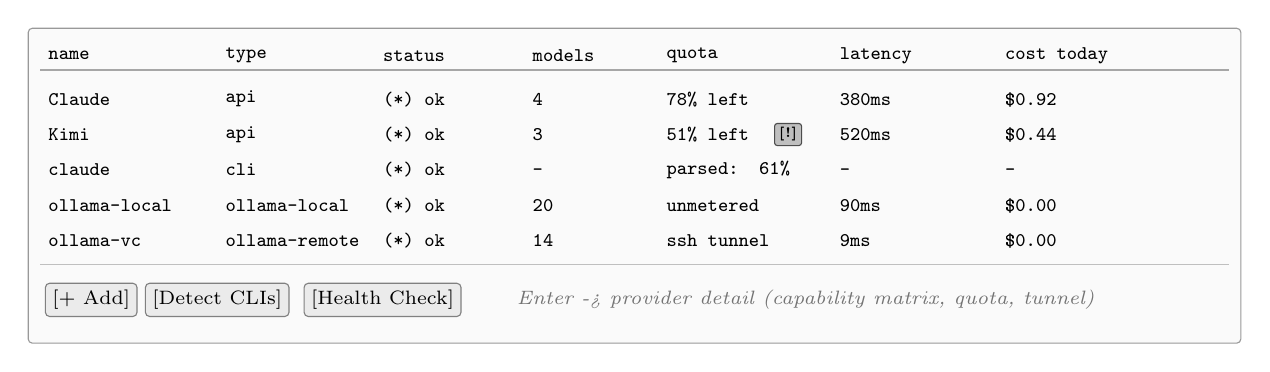
\begin{tikzpicture}[x=1cm,y=1cm]
  \draw[panel] (0,0) rectangle (15.4,4.0);

  \foreach \h/\x in {name/0.25, type/2.5, status/4.5, models/6.4, quota/8.1, latency/10.3, {cost today}/12.4} {
    \node[monob] at (\x,3.65) {\h};
  }
  \draw[black!35, line width=0.4pt] (0.15,3.47) -- (15.25,3.47);

  \foreach \n/\t/\s/\m/\q/\l/\c/\y in {%
    Claude/api/{(*) ok}/4/{78\% left}/380ms/{\$0.92}/3.1,
    Kimi/api/{(*) ok}/3/{51\% left}/520ms/{\$0.44}/2.65,
    claude/cli/{(*) ok}/-/{parsed: 61\%}/-/-/2.2,
    ollama-local/{ollama-local}/{(*) ok}/20/unmetered/90ms/{\$0.00}/1.75,
    ollama-vc/{ollama-remote}/{(*) ok}/14/{ssh tunnel}/9ms/{\$0.00}/1.3}
  {
    \node[mono] at (0.25,\y) {\n};
    \node[mono] at (2.5,\y) {\t};
    \node[mono] at (4.5,\y) {\s};
    \node[mono] at (6.4,\y) {\m};
    \node[mono] at (8.1,\y) {\q};
    \node[mono] at (10.3,\y) {\l};
    \node[mono] at (12.4,\y) {\c};
  }
  \node[warn] at (9.65,2.65) {[!]};

  \draw[black!25, line width=0.3pt] (0.15,1.0) -- (15.25,1.0);
  \foreach \b/\x in {{[+ Add]}/0.8, {[Detect CLIs]}/2.4, {[Health Check]}/4.5} {
    \node[btn] at (\x,0.55) {\b};
  }
  \node[note] at (6.2,0.55) {Enter -> provider detail (capability matrix, quota, tunnel)};
\end{tikzpicture}

\end{center}

\textbf{Provider window} (double-click): tabs \emph{Details · Models · Quota · Adapter}.

\begin{itemize}
  \item Details: type, endpoint/CLI path, key reference (never the secret — \texttt{[••• stored in keychain]},
[Change] [Test] buttons).

  \item Models: capability matrix (context, vision, tools, streaming, \$/M tok) — editable grid.
  \item Quota: plan limit, cycle, renewal date, source picker (\texttt{api/parsed/manual/estimated}),
burn graph, alert thresholds.

  \item Adapter (CLI type only): invocation template, output parser, quota parser, overlay mode.
\end{itemize}
\subsection{3.4 Rules tab}
\begin{center}
% Mission Control - Rules tab with dry-run (TUI-DESIGN 3.4)
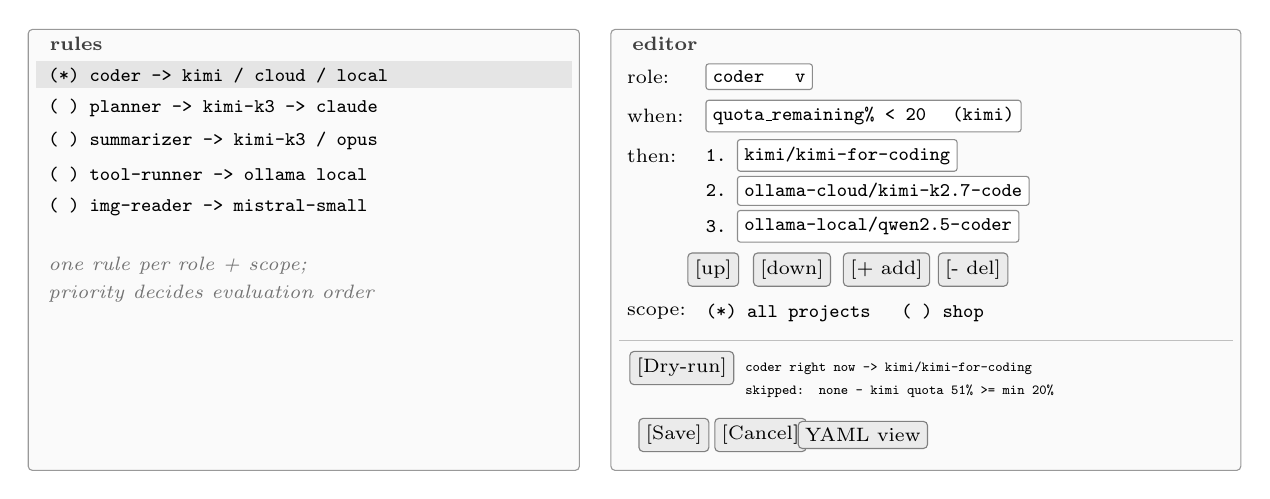
\begin{tikzpicture}[x=1cm,y=1cm]
  % ----- rule list -----
  \draw[panel] (0,0) rectangle (7.0,5.6);
  \node[panelhdr] at (0.15,5.42) {rules};
  \draw[fill=black!10, draw=none] (0.1,4.85) rectangle (6.9,5.2);
  \foreach \r/\y in {%
    {(*) coder -> kimi / cloud / local}/5.02,
    {( ) planner -> kimi-k3 -> claude}/4.6,
    {( ) summarizer -> kimi-k3 / opus}/4.18,
    {( ) tool-runner -> ollama local}/3.76,
    {( ) img-reader -> mistral-small}/3.34}
  {
    \node[mono] at (0.25,\y) {\r};
  }
  \node[note] at (0.25,2.6) {one rule per role + scope;};
  \node[note] at (0.25,2.25) {priority decides evaluation order};

  % ----- editor -----
  \draw[panel] (7.4,0) rectangle (15.4,5.6);
  \node[panelhdr] at (7.55,5.42) {editor};

  \node[lbl] at (7.6,5.0) {role:};
  \node[field, anchor=west] at (8.6,5.0) {coder \quad v};
  \node[lbl] at (7.6,4.5) {when:};
  \node[field, anchor=west] at (8.6,4.5) {quota\_remaining\% < 20 \; (kimi)};

  \node[lbl] at (7.6,4.0) {then:};
  \foreach \i/\m/\y in {1/{kimi/kimi-for-coding}/4.0, 2/{ollama-cloud/kimi-k2.7-code}/3.55, 3/{ollama-local/qwen2.5-coder}/3.1} {
    \node[mono] at (8.6,\y) {\i.};
    \node[field, anchor=west] at (9.0,\y) {\m};
  }
  \foreach \b/\x in {{[up]}/8.7, {[down]}/9.7, {[+ add]}/10.9, {[- del]}/12.0} {
    \node[btn] at (\x,2.55) {\b};
  }

  \node[lbl] at (7.6,2.0) {scope:};
  \node[mono] at (8.6,2.0) {(*) all projects \quad ( ) shop};

  \draw[black!25, line width=0.3pt] (7.5,1.65) -- (15.3,1.65);
  \node[btn] at (8.3,1.3) {[Dry-run]};
  \node[monos] at (9.1,1.3) {coder right now -> kimi/kimi-for-coding};
  \node[monos] at (9.1,1.0) {skipped: none - kimi quota 51\% >= min 20\%};
  \foreach \b/\x in {{[Save]}/8.2, {[Cancel]}/9.3, {YAML view}/10.6} {
    \node[btn] at (\x,0.45) {\b};
  }
\end{tikzpicture}

\end{center}

\begin{itemize}
  \item Left: rule list (one per role+scope); right: condition builder (comboboxes + numeric
fields) and \textbf{ordered fallback chain} editor.

  \item \textbf{Dry-run panel} evaluates the rule against live quota state and explains the choice.
  \item "YAML =>" toggle shows the canonical YAML (decision D2) with live two-way sync.
\end{itemize}
\subsection{3.5 Questions tab — Interrogation Center}
\begin{center}
% Interrogation center - Questions tab (TUI-DESIGN 3.5)
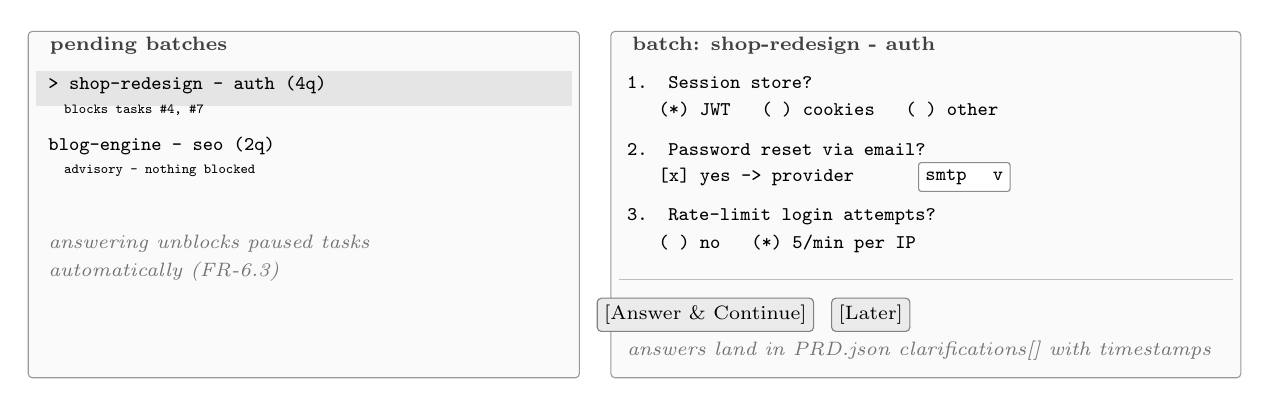
\begin{tikzpicture}[x=1cm,y=1cm]
  % pending batches
  \draw[panel] (0,0) rectangle (7.0,4.4);
  \node[panelhdr] at (0.15,4.22) {pending batches};
  \draw[fill=black!10, draw=none] (0.1,3.45) rectangle (6.9,3.9);
  \node[mono] at (0.25,3.72) {> shop-redesign - auth (4q)};
  \node[monos] at (0.45,3.4) {blocks tasks \#4, \#7};
  \node[mono] at (0.25,2.95) {blog-engine - seo (2q)};
  \node[monos] at (0.45,2.63) {advisory - nothing blocked};
  \node[note] at (0.25,1.7) {answering unblocks paused tasks};
  \node[note] at (0.25,1.35) {automatically (FR-6.3)};

  % batch detail
  \draw[panel] (7.4,0) rectangle (15.4,4.4);
  \node[panelhdr] at (7.55,4.22) {batch: shop-redesign - auth};

  \node[mono] at (7.6,3.75) {1. Session store?};
  \node[mono] at (8.0,3.4) {(*) JWT \quad ( ) cookies \quad ( ) other};
  \node[mono] at (7.6,2.9) {2. Password reset via email?};
  \node[mono] at (8.0,2.55) {[x] yes -> provider};
  \node[field, anchor=west] at (11.3,2.55) {smtp \; v};
  \node[mono] at (7.6,2.05) {3. Rate-limit login attempts?};
  \node[mono] at (8.0,1.7) {( ) no \quad (*) 5/min per IP};

  \draw[black!25, line width=0.3pt] (7.5,1.25) -- (15.3,1.25);
  \node[btn] at (8.6,0.8) {[Answer \& Continue]};
  \node[btn] at (10.7,0.8) {[Later]};
  \node[note] at (7.6,0.35) {answers land in PRD.json clarifications[] with timestamps};
\end{tikzpicture}

\end{center}

Answering unblocks paused tasks automatically (FR-6.3). "Later" keeps tasks paused but never loses the batch.

\subsection{3.6 Activity tab}
Chronological ledger stream (filterable by project/provider/type): tickets applied, rule decisions, quota events, migrations, alerts. Export CSV/JSON buttons.

\section{4. Project Window (satellite, one per project)}
Opened from Projects tab (\texttt{Enter}) or \texttt{maestro project open shop}.

\begin{center}
% Project window with task DAG (TUI-DESIGN 4)
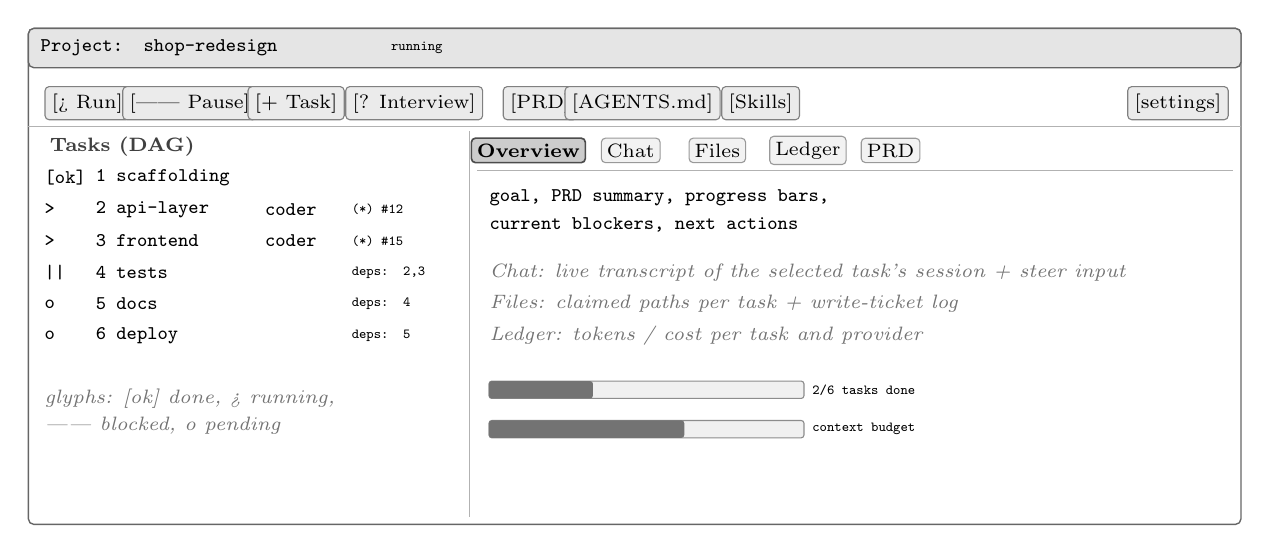
\begin{tikzpicture}[x=1cm,y=1cm]
  \draw[win] (0,0) rectangle (15.4,6.3);
  \draw[titlebar] (0,5.8) rectangle (15.4,6.3);
  \node[monob] at (0.15,6.05) {Project: shop-redesign};
  \node[monos] at (4.6,6.05) {running};

  % toolbar
  \foreach \b/\x in {{[> Run]}/0.75, {[|| Pause]}/2.05, {[+ Task]}/3.4, {[? Interview]}/4.9, {[PRD]}/6.5, {[AGENTS.md]}/7.8, {[Skills]}/9.3} {
    \node[btn] at (\x,5.35) {\b};
  }
  \node[btn] at (14.6,5.35) {[settings]};
  \draw[black!30, line width=0.4pt] (0,5.05) -- (15.4,5.05);

  % ---- left: task DAG ----
  \node[panelhdr] at (0.15,4.8) {Tasks (DAG)};
  \foreach \s/\n/\r/\extra/\y in {%
    {[ok]}/{1 scaffolding}//{}/4.4,
    {>}/{2 api-layer}/coder/{(*) \#12}/4.0,
    {>}/{3 frontend}/coder/{(*) \#15}/3.6,
    {||}/{4 tests}/{}/{deps: 2,3}/3.2,
    {o}/{5 docs}/{}/{deps: 4}/2.8,
    {o}/{6 deploy}/{}/{deps: 5}/2.4}
  {
    \node[mono] at (0.2,\y) {\s};
    \node[mono] at (0.85,\y) {\n};
    \node[mono] at (3.0,\y) {\r};
    \node[monos] at (4.1,\y) {\extra};
  }
  \node[note] at (0.2,1.6) {glyphs: [ok] done, > running,};
  \node[note] at (0.2,1.25) {|| blocked, o pending};
  \draw[black!30, line width=0.4pt] (5.6,0.1) -- (5.6,5.0);

  % ---- right: tabs ----
  \node[tabsel] at (6.35,4.75) {Overview};
  \foreach \t/\x in {Chat/7.65, Files/8.75, Ledger/9.9, PRD/10.95} {
    \node[tab] at (\x,4.75) {\t};
  }
  \draw[black!30, line width=0.4pt] (5.7,4.5) -- (15.3,4.5);
  \node[mono] at (5.85,4.15) {goal, PRD summary, progress bars,};
  \node[mono] at (5.85,3.8) {current blockers, next actions};
  \node[note] at (5.85,3.2) {Chat: live transcript of the selected task's session + steer input};
  \node[note] at (5.85,2.8) {Files: claimed paths per task + write-ticket log};
  \node[note] at (5.85,2.4) {Ledger: tokens / cost per task and provider};

  % progress bars
  \gauge{5.85}{1.6}{4.0}{0.33}{2/6 tasks done}
  \gauge{5.85}{1.1}{4.0}{0.62}{context budget}
\end{tikzpicture}

\end{center}

\begin{itemize}
  \item Left: \textbf{TreeView of the DAG} — state glyphs ([ok] done, > running, || paused/blocked,
o pending), role, live session id. Selecting a task binds the right-side tabs.

  \item Toolbar [?] \textbf{Interview} opens the clarification form for this project; \textbf{AGENTS.md}
previews the generated file with diff on regeneration; \textbf{Skills} opens the suggestion/install panel.

  \item Right-side tabs (splitter draggable): Overview / Chat / Files / Ledger / (+PRD view).
\end{itemize}
\subsection{4.1 Chat / Session view (the heart of single-model interaction)}
\begin{center}
% Chat / session view (TUI-DESIGN 4.1)
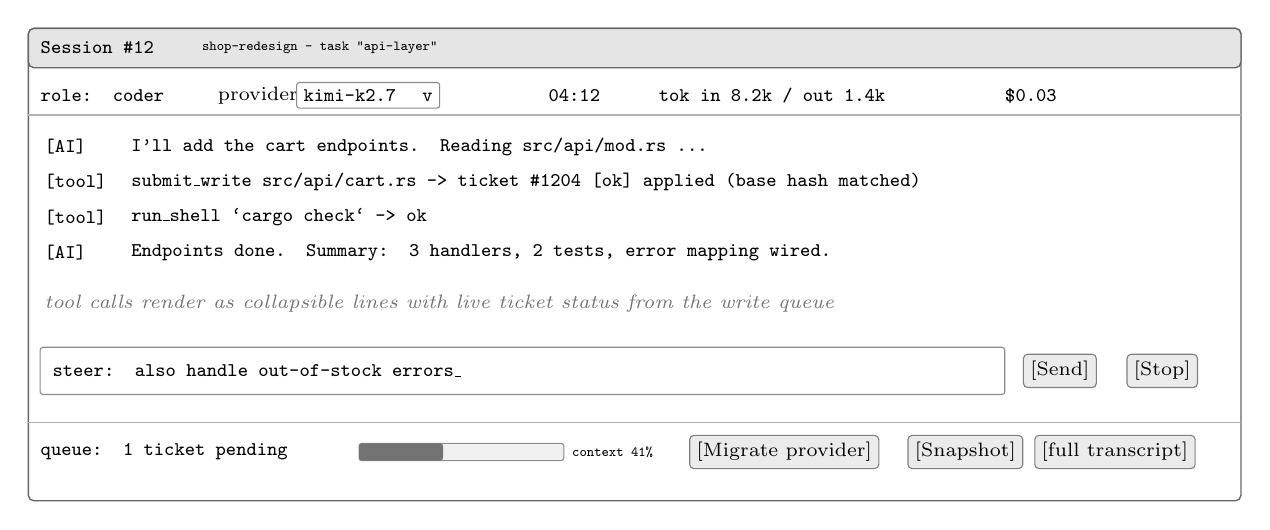
\begin{tikzpicture}[x=1cm,y=1cm]
  \draw[win] (0,0) rectangle (15.4,6.0);
  \draw[titlebar] (0,5.5) rectangle (15.4,6.0);
  \node[monob] at (0.15,5.75) {Session \#12};
  \node[monos] at (2.2,5.75) {shop-redesign - task "api-layer"};

  % status line
  \node[mono] at (0.15,5.15) {role: coder};
  \node[lbl] at (2.4,5.15) {provider:};
  \node[field, anchor=west] at (3.4,5.15) {kimi-k2.7 \; v};
  \node[mono] at (6.6,5.15) {04:12};
  \node[mono] at (8.0,5.15) {tok in 8.2k / out 1.4k};
  \node[mono] at (12.4,5.15) {\$0.03};
  \draw[black!30, line width=0.4pt] (0,4.9) -- (15.4,4.9);

  % transcript
  \foreach \tag/\txt/\y in {%
    {[AI]}/{I'll add the cart endpoints. Reading src/api/mod.rs ...}/4.5,
    {[tool]}/{submit\_write src/api/cart.rs -> ticket \#1204 [ok] applied (base hash matched)}/4.05,
    {[tool]}/{run\_shell `cargo check` -> ok}/3.6,
    {[AI]}/{Endpoints done. Summary: 3 handlers, 2 tests, error mapping wired.}/3.15}
  {
    \node[monob] at (0.2,\y) {\tag};
    \node[mono] at (1.3,\y) {\txt};
  }
  \node[note] at (0.2,2.5) {tool calls render as collapsible lines with live ticket status from the write queue};

  % steer input
  \draw[field] (0.15,1.35) rectangle (12.4,1.95);
  \node[mono] at (0.3,1.65) {steer: also handle out-of-stock errors\_};
  \node[btn] at (13.1,1.65) {[Send]};
  \node[btn] at (14.4,1.65) {[Stop]};

  % footer
  \draw[black!30, line width=0.4pt] (0,1.0) -- (15.4,1.0);
  \node[mono] at (0.15,0.62) {queue: 1 ticket pending};
  \gauge{4.2}{0.51}{2.6}{0.41}{context 41\%}
  \foreach \b/\x in {{[Migrate provider]}/9.6, {[Snapshot]}/11.9, {[full transcript]}/13.8} {
    \node[btn] at (\x,0.62) {\b};
  }
\end{tikzpicture}

\end{center}

\begin{itemize}
  \item Transcript: RichTextField, streamed; tool calls rendered as collapsible lines with
ticket status pulled live from the write queue.

  \item Provider combobox: switch model mid-session -> triggers structured-snapshot migration
(decision D5), with confirmation.

  \item Bottom bar: queue state for this session's tickets, context-window usage, actions
(Migrate / Snapshot / open full transcript in markdown viewer).

\end{itemize}
\section{5. Quick Chat (single LLM, no project)}
\texttt{Ctrl+Q} or Sessions -> Quick Chat. A lightweight window for ad-hoc conversation:

\begin{center}
% Quick Chat window (TUI-DESIGN 5)
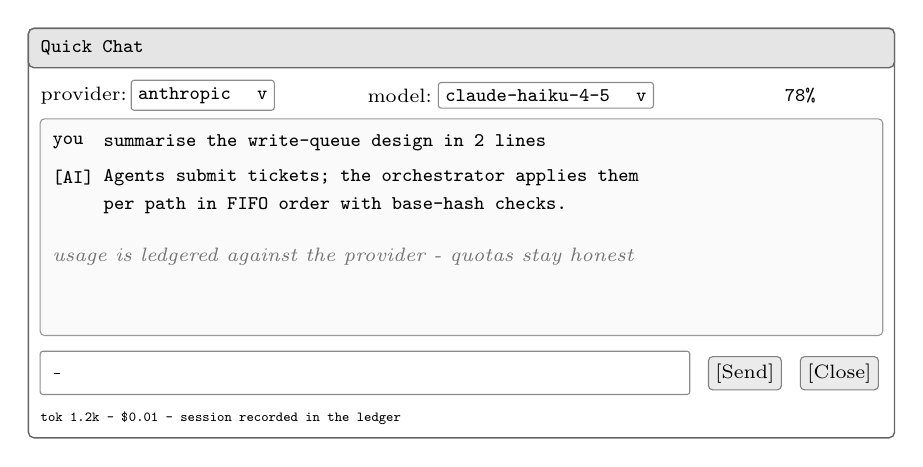
\begin{tikzpicture}[x=1cm,y=1cm]
  \draw[win] (0,0) rectangle (11.0,5.2);
  \draw[titlebar] (0,4.7) rectangle (11.0,5.2);
  \node[monob] at (0.15,4.95) {Quick Chat};

  \node[lbl] at (0.15,4.35) {provider:};
  \node[field, anchor=west] at (1.3,4.35) {anthropic \; v};
  \node[lbl] at (4.3,4.35) {model:};
  \node[field, anchor=west] at (5.2,4.35) {claude-haiku-4-5 \; v};
  \node[mono] at (9.6,4.35) {78\%};

  \draw[panel] (0.15,1.3) rectangle (10.85,4.05);
  \node[monob] at (0.3,3.75) {you};
  \node[mono] at (0.95,3.75) {summarise the write-queue design in 2 lines};
  \node[monob] at (0.3,3.3) {[AI]};
  \node[mono] at (0.95,3.3) {Agents submit tickets; the orchestrator applies them};
  \node[mono] at (0.95,2.95) {per path in FIFO order with base-hash checks.};
  \node[note] at (0.3,2.3) {usage is ledgered against the provider - quotas stay honest};

  \draw[field] (0.15,0.55) rectangle (8.4,1.1);
  \node[mono] at (0.3,0.82) {\_};
  \node[btn] at (9.1,0.82) {[Send]};
  \node[btn] at (10.3,0.82) {[Close]};
  \node[monos] at (0.15,0.25) {tok 1.2k - \$0.01 - session recorded in the ledger};
\end{tikzpicture}

\end{center}

\begin{itemize}
  \item Token usage is still ledgered against the provider (quotas stay honest).
  \item \textbf{Promote to task}: converts the chat into a project task with the transcript as
context seed. Attach ([clip]) adds files/images for vision-capable models.

\end{itemize}
\section{6. Settings}
Menu Tools -> Settings (\texttt{F10}). Modal window: left Accordion/ListBox of sections, right side shows the section's form. \textbf{[Save] applies to TOML live; [Defaults] resets.}

\subsection{Settings inventory}
\begin{small}
\begin{tabularx}{\linewidth}{lX}
\toprule
Section & Keys \\
\midrule
\textbf{General} & workspace root, default project template, language/locale, autostart behavior, check for updates \\
\textbf{Appearance} & theme (dark/light/custom), true-color toggle, font-size hint, dashboard density, confirm-on-exit \\
\textbf{Parallelism} & global session cap (default: CPU heuristic, D6), per-provider concurrency limits, write-queue batch size, per-project fairness quota \\
\textbf{Quotas \& alerts} & warn thresholds (default 80/95\%), alert action (notify / auto-switch rule / pause role), burn-rate window, renewal reminders \\
\textbf{Rules} & default question mode (thorough/balanced/minimal — FR-6.4), unmatched-role behavior (ask / cheapest / fail), rule conflict precedence \\
\textbf{Secrets} & backend: keychain <-> encrypted vault, vault path, master-password timeout, env-var passthrough allow-list \\
\textbf{Sandbox \& security} & shell allow-list per project, network access for tool-runner, overlay mode for CLI adapters (D3), redaction level \\
\textbf{Projects} & default DAG parallelism, auto git checkpoints on/off, AGENTS.md regeneration policy (ask/auto), skill registry paths \\
\textbf{Storage} & config dir, SQLite path, transcript retention days, ledger export format, backup on exit \\
\textbf{Notifications} & TUI popups on/off, OS toast on/off, sound, quiet hours \\
\textbf{Keybindings} & full remapping table (searchable) \\
\textbf{Headless/API} & default \texttt{--json}, NDJSON watch toggle, exit-code verbosity \\
\textbf{Advanced} & log level, event-bus buffer size, experimental flags, reset all state \\
\bottomrule
\end{tabularx}
\end{small}

\section{7. Interaction Flows}
\subsection{7.1 First run (onboarding wizard, runs once)}
\begin{itemize}
  \item Welcome -> pick workspace root \& theme.
  \item \textbf{Detect providers}: scans PATH for \texttt{claude}/\texttt{codex}/\texttt{gemini}/\texttt{ollama}, probes
\texttt{localhost:11434}; shows found list with checkboxes.

  \item \textbf{Add API providers}: endpoint + key (stored to keychain, FR-2) -> auth test ->
model discovery.

  \item \textbf{Quota setup}: for each provider pick source (auto / manual budget) + plan limits.
  \item \textbf{Default rules}: proposed from capabilities (e.g. tool-runner -> ollama local);
user confirms in the rule editor.

  \item Done -> Mission Control. \texttt{maestro config doctor} summary shown.
\end{itemize}
\subsection{7.2 New project}
\begin{itemize}
  \item \texttt{Ctrl+N} -> wizard: name, dir, stack, git init.
  \item \textbf{Interview} (interrogator role, FR-6): batched forms; answers stream into PRD.json.
  \item Maestro drafts \textbf{PRD.md} -> user reviews in markdown tab -> approve -> PRD.json compiled.
  \item \textbf{AGENTS.md + skill suggestions} generated; user checks which skills to install.
  \item \textbf{Task DAG proposal} shown in the project's tree; user edits/reorders -> \textbf{Run}.
  \item Sessions spawn per rule routing; dashboard shows them; questions may reappear
mid-flight in the app bar ([?] badge).

\end{itemize}
\subsection{7.3 Quota-exceeded event (no user action needed)}
\begin{itemize}
  \item Provider returns 429 / parsed quota hits threshold -> rule re-evaluates (FR-3.3).
  \item Session migrates via structured snapshot (D5); transcript gains a
\texttt{── migrated kimi-k2.7 -> glm-5.2 ──} marker.

  \item App bar [!] badge + notification; Activity tab records the decision and its reason.
\end{itemize}
\subsection{7.4 Steering a running agent}
Open session window -> type in steer box -> message injected into agent loop. \texttt{■ Stop} pauses with snapshot; resume continues with context intact.

\section{8. Keybindings (defaults, remappable)}
\begin{small}
\begin{tabularx}{\linewidth}{lX}
\toprule
Key & Action \\
\midrule
\texttt{Ctrl+Q} & Quick Chat \\
\texttt{Ctrl+N} & New Project \\
\texttt{F10} & Settings \\
\texttt{F1..F6} & Mission Control tabs (Dashboard…Activity) \\
\texttt{Ctrl+Enter} & Send (chat/steer) \\
\texttt{Ctrl+P} & Command palette (jump to project/provider/rule/session) \\
\texttt{Ctrl+D} & Dry-run rule under cursor \\
\texttt{Ctrl+T} & Tile all satellite windows \\
\texttt{Esc} & Close dialog / blur input \\
\texttt{?} & Shortcuts overlay \\
\bottomrule
\end{tabularx}
\end{small}

\section{9. AppCUI Control Mapping}
\begin{small}
\begin{tabularx}{\linewidth}{lX}
\toprule
Need & AppCUI control \\
\midrule
Tabs everywhere & \texttt{Tab} \\
Sessions/providers/projects tables & \texttt{ListView} (columns, sort) \\
Task DAG & \texttt{TreeView} + custom glyphs \\
Quota gauges & \texttt{ProgressBar} + \texttt{GraphView} (burn sparklines) \\
PRD view & \texttt{Markdown} viewer \\
Chat transcript & \texttt{RichTextField} (read-only, appended) \\
Steer/chat input & \texttt{TextField} (multiline) + \texttt{Button} \\
Rule builder & \texttt{ComboBox}, \texttt{NumericField}, \texttt{ListBox} + up/down \\
Settings sections & \texttt{Accordion} / \texttt{ListBox} + panel swap \\
Project window panes & \texttt{Splitter} \\
Global status & \texttt{AppBar} segments \\
Wizards/onboarding & modal \texttt{Window}s + \texttt{Button}s, \texttt{CheckBox}, \texttt{RadioButton} \\
Questions forms & generated \texttt{RadioButton}/\texttt{CheckBox}/\texttt{TextField}/\texttt{DatePicker} \\
Toasts/alerts & notification dialogs + app bar badges \\
Theming & built-in themes, true-color \\
\bottomrule
\end{tabularx}
\end{small}

\section{10. Window Inventory}
\begin{small}
\begin{tabularx}{\linewidth}{lXX}
\toprule
Window & Kind & Opened from \\
\midrule
Mission Control & main (maximized) & startup \\
Onboarding wizard & modal & first run / Tools \\
Project window & satellite & Projects tab, \texttt{maestro project open} \\
Session/Chat window & satellite & dashboard/chat tab, Quick Chat promote \\
Quick Chat & satellite & \texttt{Ctrl+Q} \\
Provider window & modal-ish & Providers tab \\
Provider wizard & modal & Providers -> Add \\
Rule editor & tab panel & Rules tab \\
Interrogation form & panel/modal & Questions tab, app bar [?] \\
Settings & modal & \texttt{F10} \\
Transcript viewer & satellite & session -> [log] full \\
File/picker dialogs & stock AppCUI & wizards \\
\bottomrule
\end{tabularx}
\end{small}

\end{document}
